
\chapter{Introduction} \label{ch:Introduction}
\graphicspath{{chapter1_ys/}}
\minitoc


The physics of plasma turbulence is among the most important problems in fusion research and has been extensively studied experimentally and theoretically. However, a global physical picture is still lacking. The contribution of this thesis is to explore trends of turbulence properties over a broad range of plasma conditions. This is different from the previous work, which is conventionally based on a limited number of dedicated experiments under specific plasma conditions. With the increasing size of databases over the past few decades, techniques have been developed to detect patterns in large data sets. It is this type of approach that we have intended to transfer to the investigation of turbulence in fusion plasmas, based on diagnostic measurements that are sensitive to turbulent fluctuations.

In particular, in this thesis a parametrization method is developed for frequency spectra obtained from reflectometry, for a systematic turbulence study in tokamak plasmas. The method is applied to a large database from the Tore Supra tokamak, in order to extract patterns (trends, clusters) reflecting interesting underlying physics across a wide range of plasma conditions. The statistical approach is able to provide useful information which is difficult to obtain through the traditional shot-to-shot analysis.

This chapter provides an introduction to the topics that the present thesis is concerned with. Section \ref{sec:energy_issues} touches upon the background of the worldwide energy problem and discusses a number of alternative solutions for sustainable energy generation. Fusion turns out to be one possible solution, where one promising experimental configuration is the tokamak device, which is discussed in section \ref{sec:tokamak}. One of the main obstacles on the route to fusion energy is the problem of turbulent energy transport. Solving this problem requires a better understanding and control of the micro-instabilities responsible for the turbulent activity. This serves as the basic motivation of this thesis, as presented in section \ref{sec:motivation_thesis}.


\section{Energy issues and solutions} \label{sec:energy_issues}


The energy problem is related to a scarceness of resources as well as environmental problems, affecting countries all over the world. These issues will become even more severe in the future considering the continuous increase and development of world population. Several alternative energy sources are being developed, which are sustainable and environmentally friendly. Fusion energy is one of them, with magnetic confinement fusion currently the main research avenue.


\subsection{Demand for new energy sources}


%%%%%%%%%%%%%%%%%%%%
\begin{figure}[h]
\begin{centering}
\includegraphics[scale=0.55]{energy2017.png}
\par\end{centering}
\caption{World energy consumption in 2017 \cite{BP_2017_Energy}.}
\label{fig:energy2017}
\end{figure}
%%%%%%%%%%%%%%%%%%%%

Fossil fuels (coal, oil and natural gas) have greatly influenced our lives for a long time and still play a dominant role in the current world energy consumption, as shown in figure \ref{fig:energy2017}. However, fossil fuels not only have a harmful effect on the environment, e.g., air pollution and the global warming by greenhouse gases, but also face the problem of exhaustion \cite{Abas_2015_Fs}. It has been estimated that coal, oil and natural gas resources will be depleted within about 110, 50 and 50 years, respectively \cite{Shafiee_2009_NP}. As a result, increasing efforts are devoted to development and implementation of renewable energy \cite{Akella_2009_RE}, which are economic viable. However, the main renewable energy sources, including hydro-energy, solar, wind, geothermal and biomass \cite{Fridleifsson_2001_RSER, Momirlan_2005_IJHE, Jacobson_2011_EP}, are limited by the local natural conditions and, as a result, their applicability depends on one region to another\cite{Panwar_2011_RSER}. Other problems are related to storage (due to intermittency) and transport of energy \cite{Agbossou_2004_IEEE, Kaldellis_2007_En, Rentizelas_2009_RSER}.





On the other hand, nuclear energy based on the mass-energy equation $E = mc^2$ is an alternative option and there are basically two approaches: fission and fusion, as shown in figure \ref{fig:binding_energy}. While fission involves the splitting of heavy atomic nuclei, fusion of light nuclei also releases energy, as shown in  figure \ref{fig:binding_energy}. Fission energy has been used in the industrial electricity generation for many years, and it does not generate greenhouse gases. However, the radioactive nuclear waste and risk of nuclear accidents, such as the Fukushima event \cite{Bolsunovsky_2011_JER}, are reducing its acceptability. In addition, considering the limited reserves of uranium, fission has been estimated to be usable for limited time before exhaustion \cite{Dittmar_2013_STE}.


%%%%%%%%%%%%%%%%%%%%
\begin{figure}[h]
\begin{centering}
\includegraphics[scale=0.25]{binding_energy.png}
\par\end{centering}
\caption{Binding energy per nucleon evolves with the atomic mass number.}
\label{fig:binding_energy}
\end{figure}
%%%%%%%%%%%%%%%%%%%%


In contrast, fusion energy is clean, with low radioactivity \cite{Khvesyuk_2002_PPCF} and also without emission of greenhouse gases. The basic fuel reserves are as good as endless: deuterium and tritium come from the ocean and the self-breeding from $_3\mathrm{Li}^6$ (abundant in the earth's crust), respectively. The mere resources on the earth can already support the energy consumptions of humans for at least thousands of years \cite{Ongena_2012_FST}.


\subsection{Principles of fusion} \label{sec:principles_fusion}


Although any combination of light nuclei could lead to the realization of fusion reactions, the most effective ones with the largest cross-sections are \cite{Freidberg_2007_Plasma}:%
%%%%%%%%%%%%%%%%%%%%
\begin{eqnarray}
    \mathrm{D} &+& \mathrm{T} \rightarrow \alpha + \mathrm{n} + \mathrm{17.6\ MeV}, \\
    \mathrm{D} &+& \mathrm{D} \rightarrow (50\%)\ \mathrm{He^3} + \mathrm{n} + \mathrm{3.27\ MeV}, \\
    \mathrm{D} &+& \mathrm{D} \rightarrow (50\%)\ \mathrm{T} + \mathrm{p} + \mathrm{4.03\ MeV}, \\
    \mathrm{D} &+& \mathrm{He^3} \rightarrow \alpha + \mathrm{p} + \mathrm{18.3\ MeV}.
\end{eqnarray}
%%%%%%%%%%%%%%%%%%%%
\noindent Here, D is deuterium ($^2\mathrm{H}$), T is tritium ($^3\mathrm{H}$), $^3\mathrm{He}$ is helium-3, $\alpha$ is the helium nucleus (alpha particle, $_2^4\mathrm{He}^{2+}$), n is neutron, p is proton.

In fusion reactions, the reaction rate is proportional to the cross-section for the different reactions. The cross-section is strongly affected by the reaction temperature, as shown in figure \ref{fig:cross_section_vs_energy}. In order to obtain a large cross-section, thus an effective reactivity, the temperature should be at least tens of keV, corresponding to $\sim$ 100 millions $^\circ$C. At such high temperatures, the kinetic energy per particle becomes much larger than its ionization energy (order of eV), so the reaction fuel constituents no longer form neutral atoms but exist in the plasma state.


%%%%%%%%%%%%%%%%%%%%
\begin{figure}[h]
\begin{centering}
\includegraphics[scale=0.6]{cross_section_vs_energy.png}
\par\end{centering}
\caption{Cross -section of some basic fusion reactions as a function of the particle energy. Reprinted from \cite{Bittencourt_2004_Plasma}.}
\label{fig:cross_section_vs_energy}
\end{figure}
%%%%%%%%%%%%%%%%%%%%


However, the difficulty is not the fusion reaction itself, which has already been achieved by the explosion of hydrogen bombs, but an effective control of the reaction process to obtain a stable and continuous output of energy. Therefore the confinement of the reaction fuel is of fundamental importance. Studies have shown that, in order to realize a controlled self-sustaining reaction (burning) of the fuel, the product of the fuel density ($n$) and the energy confinement time ($\tau_{E}$) must satisfy the so-called ignition condition \cite{Wesson_1997_Tokamaks}:%
%%%%%%%%%%%%%%%%%%%%
\begin{equation}
    n\tau_E > 1.5 \times 10^{20}\ m^{-3}s,
\end{equation}
%%%%%%%%%%%%%%%%%%%%
\noindent given that the optimal temperature is realized. On the other hand, in terms of the power balance, the loss power is balanced by the externally supplied power plus the $\alpha-$particle power: $P_L = P_H + P_{\alpha}$. The power amplification factor $Q$ is a measure of reactor performance:%
%%%%%%%%%%%%%%%%%%%%
\begin{equation} \label{eq:Q}
   Q = \frac{P_{\alpha}}{P_H}.
\end{equation}
%%%%%%%%%%%%%%%%%%%%
\noindent Here, $Q = 1$ means that 20$\%$ of the applied heating power comes from the $\alpha-$particles. At ignition, $P_H$ should be zero and $Q \rightarrow \infty$, thus all the loss power is compensated by the $\alpha-$particle power.

There are mainly two distinct methods to approach a self-burning fusion reaction: magnetic confinement fusion (MCF) \cite{Artsimovich_1972_NF} and inertial confinement fusion (ICF) \cite{Miller_2004_NF_NIF, Craxton_2015_PoP}. MCF aims at increasing the confinement time of low-density plasmas using magnetic fields, whereas in ICF the fuel is heated and compressed using a high-power short laser pulse. ICF has been studied for instance at the National Ignition Facility (NIF) \cite{Moses_2016_FST}, but the ignition condition has not been reached due to various unresolved problems, such as controlling the symmetry of the imploding fuel \cite{Michel_PRL_2009}, Rayleigh-Taylor instabilities \cite{Nagel_2017_PoP}, shockwave convergence \cite{Ma_2016_IEEE}, etc. In addition, the $Q$ value obtained in ICF has not met expectations so far \cite{Ross_2015_PRE, Le-Pape_2018_PRL}. On the other hand, in MCF there has been significant progress towards the ignition condition and the $Q$ value has been steadily raised. Confinement times of the order of seconds and $Q > 1$ have been obtained\cite{Romanelli_2015_NF}. This thesis is situated in the area of MCF, which is the more promising fusion scheme for the near future.


\section{Tokamaks} \label{sec:tokamak}


In the study of MCF, many different devices with different magnetic geometries have been invented since 50's. Among the other devices such as magnetic mirrors, stellarators, and reversed-field pinches, the tokamak has shown the most promising performance towards realising net fusion power generation. This section covers only some general concepts of tokamaks.


\subsection{Motions of charged particles in magnetic fields}


As mentioned before, the fusion reaction fuels are ionized to form the state of plasma at high temperature. At that point, the motion of the charges plasma particles, i.e. electrons and ions, is no longer predominately determined by short-range Coulomb collisions between the particles, but by long-range electromagnetic forces. This has inspired scientists to utilize external magnetic fields to confine the fuel (i.e., the plasmas).

Therefore, in order to understand the confinement performance of tokamaks, the first ingredient is the motion of charged particles in external magnetic fields.

The theory of magnetohydrodynamics (MHD) \cite{Goldston_1995_Plasma, Freidberg_2007_Plasma} and kinetic theory \cite{Stix_1992_Waves, Bittencourt_2004_Plasma} have been developed to describe the complex plasma behavior in the presence of external magnetic fields. In the MHD model, a plasma is regarded as a fluid in the presence of electromagnetic fields. Kinetic theory is based on the distribution function in six-dimensional phase space to completely describe the plasma motion from a statistical point-of-view.

Here, for simplicity, a single particle in a uniform magnetic field is considered, to capture the most important features of the motion. Figure \ref{fig:gyro_motion} shows the helical motion of a positively charged particle in an external uniform magnetic field ($\textbf{B}$). In the direction parallel to $\textbf{B}$, the parallel velocity of the particle ($\boldsymbol{\upsilon}_{\parallel}$) is constant. In the direction perpendicular, the particle undergoes a gyro-motion with velocity ($|\boldsymbol{\upsilon}_{\perp}|$). The cyclotron frequency ($\omega_{c}$) of the perpendicular motion is%
%%%%%%%%%%%%%%%%%%%%
\begin{equation}
  \omega_{cs} = \frac{q_s B}{m_{s}},
\end{equation}
%%%%%%%%%%%%%%%%%%%%
\noindent where $q_s$ and $m_s$ are the charge and mass of the particle, and $B$ is the magnitude of the magnetic fields. The gyro-radius (Larmor radius) is%
%%%%%%%%%%%%%%%%%%%%
\begin{equation}
  \rho_s = \frac{m_s \upsilon_{\perp} }{q_s B},
\end{equation}
%%%%%%%%%%%%%%%%%%%%
\noindent where $\upsilon_{\perp}$ is the magnitude of the velocity perpendicular to $\textbf{B}$, with $s = e, i$ for electron and ion. As a result, the composite motion of the particle is a helical motion around $\textbf{B}$.


%%%%%%%%%%%%%%%%%%%%
\begin{figure}[h]
\begin{centering}
\includegraphics[scale=0.3]{gyro_motion.png}
\par\end{centering}
\caption{Illustration of the gyro-motion of the charged particles in a uniform magnetic field. Copyright@ 2004 Pearson Education, Inc., publishing as Addison Wesley.}
\label{fig:gyro_motion}
\end{figure}
%%%%%%%%%%%%%%%%%%%%


\subsection{Magnetic configurations}


Since the charged particles tend to gyrate around the magnetic lines of force, they are limited in their motion across the magnetic field. Hence, the simplest idea to confine a plasma is to use a linear device in cylindrical shape with strong magnetic fields generated by the external coils to confine the particles. However, there would still be particles losses at both ends of such a device, even when the magnetic fields around the open ends have been further strengthened to help confine the particles, like in magnetic mirrors.

The solution is to connect the ends of the device by bending the linear (cylindrical) configuration into a torus. The transformation of the device shape avoids particle losses at the two ends, thus greatly enhancing the confinement performance. However, several other forms of particle losses exist, i.e. particle drifts due to the toroidal geometry of the device. Therefore, to further compensate the particle drifts, the magnetic fields have to be twisted to become helical field lines. Moreover, further studies have shown that the twisted magnetic fields could effectively reduce several instabilities, thus further improving the confinement.


There are two methods to generate helical magnetic fields. One straightforward way is to construct helical magnetic coils, and the corresponding apparatus is called \emph{stellarator}. However, the construction of such magnetic coils needs extremely high accuracy and it is very complicated to guarantee the precise magnetic fields \cite{Motojima_2000_NF_LHD}. The tokamak is the other concept to realize the required magnetic configuration through large plasma currents, as shown in figure \ref{fig:magnetic_field}. First, in figure \ref{fig:magnetic_field} (a), the toroidal magnetic field ($B_{\phi}$) is generated by external magnetic coils. Then, in figure \ref{fig:magnetic_field} (b), the poloidal magnetic fields ($B_{\theta}$) are induced by large toroidal plasma currents ($I_p$). The resulting total helical magnetic field $B_{tot}$, the composition of $B_{\phi}$ and $B_{\theta}$, is shown in figure \ref{fig:magnetic_field} (c). Note that in tokamaks, $I_p$ is usually very large (in the order of MA). Nevertheless, the self-generated $B_{\theta}$ ($\sim$ tens of Gauss) is much smaller than $B_{\phi}$ (a few Tesla). Accordingly, the charged particles in tokamaks move along the magnetic field lines around the torus and thus are confined, to a large extent, in the device.


%%%%%%%%%%%%%%%%%%%%
\begin{figure}[h]
\begin{centering}
\includegraphics[scale=0.7]{B.png}
\par\end{centering}
\caption{Composition of the total helical magnetic fields $B_{tot}$ (c) in tokamaks from (a) toroidal $B_{\phi}$  and (b) poloidal $B_{\theta}$ magnetic fields.}
\label{fig:magnetic_field}
\end{figure}
%%%%%%%%%%%%%%%%%%%%

From the analysis above, the magnetic configuration of a tokamak is crucial to its confinement performance. Therefore, it is important to further understand the complicated magnetic fields generated by the varying $B_{\phi}$ and $B_{\theta}$ with respect to spatial coordinates. Before that, some definitions of the spatial geometry are necessary, as shown in figure \ref{fig:cross_section}. A simple circular plasma cross-section has been considered here to illustrate the spatial coordinates and parameters. The directions of $\phi$, $\theta$, $R$ indicate the toroidal, poloidal and radial coordinate, respectively. The plasma major radius ($R_p$) is defined as the distance between the plasma center ($O$) and the central axis ($L_0$). The plasma minor radius ($a$) is just the distance between the plasma edge and the center. According to the relative ratio between $R_p$ and $a$, the tokamaks can be further categorized into the conventional tokamaks ($R_p \gg a$) and the spherical tokamaks ($R_p \sim a$). Most of the tokamak fusion studies have been focused on the conventional tokamaks, while the study on the spherical tokamaks has been advocated in recent years due to their compactness and thus lower cost, although normally higher magnetic fields are required. In the plane of the poloidal cross-section ($\phi = $ constant), the plasma position can be described by two different coordinate systems: cylindrical coordinates ($R, Z$) ($0 \leq R < +\infty, -\infty < Z < +\infty$) and polar coordinates ($r, \theta$) ($0 \leq r < +\infty, 0 \leq \theta < 2\pi$). These provide the absolute spatial position and the relative position w.r.t. the plasma center, respectively. For many studies focusing on the poloidal cross-section and assuming toroidal symmetry, the relative positions ($r, \theta$) are more convenient to describe the plasma position. Specifically, for the study only on the mid-plane ($Z = 0$), the one-dimensional normalized radial position can be expressed as $\rho = rcos(\theta)/a$. Then, since the magnetic field decreases from the central axis ($L_0$) towards the outer boundary ($B_{\phi} \propto 1/R$), $\rho < 0$ and $\rho > 0$ are referred as the high-field side (HFS) and the low-field side (LFS), respectively.


%%%%%%%%%%%%%%%%%%%%
\begin{figure}[h]
\begin{centering}
\includegraphics[scale=0.4]{cross_section.png}
\par\end{centering}
\caption{Illustration of a simple circular cross-section of tokamaks to define the basic parameters in tokamak configurations.}
\label{fig:cross_section}
\end{figure}
%%%%%%%%%%%%%%%%%%%%


We continue our understanding of the tokamak magnetic configuration through the safety factor $q$. From figure \ref{fig:magnetic_field} (c), the magnetic field lines (or the charged particles) follow a helical trajectory when travelling around the torus. When the field lines (or particles) return to their initial positions after $m$ laps in the toroidal direction and $n$ laps in the poloidal direction, the \emph{safety factor} is defined as: $q = m/n$. The safety factor is a measurement of twist or helicity of the magnetic fields, i.e. weaker twist leads to larger $q$. In general, higher $q$ leads to better stability of operation, explaining the origin of the term `safety factor'. However, the optimal operation scenarios usually have moderate values of $q$, since some mechanisms of confinement and instabilities must be balanced. In normal equilibrium states, $q$ increases monotonously from the plasma center towards the plasma edge and is symmetrical with respect to the plasma center. Then, the radial profile of $q$ can be approximated by%
%%%%%%%%%%%%%%%%%%%%
\begin{equation}
q(r) = \frac{2{\pi}r^2B_{\phi}}{\mu_0I(r)R},
\end{equation}
%%%%%%%%%%%%%%%%%%%%
\noindent where $\mu_0$ is the vacuum permeability. In the $q$ profile, the radial positions with rational numbers in the safety factor ($q = 1/1,2/1,3/2,4/3,...$) are important, since MHD instabilities such as magnetic islands and tearing modes can form at these locations under certain conditions. Specifically, the $q = 1$ position (surface) is related to the sawtooth instabilities \cite{Chapman_2011_PPCF_ST_review}, which is a quasi-periodic crash and subsequent relaxation of the core plasma temperature affecting the plasma confinement. However, sometimes accurate measurement of the complete $q$ profile is not available and only the edge safety factor ($q_{\psi} = q(a)$) is measured. The edge safety factor $q_{\psi}$ is one of the most important dimensionless parameters determining confinement performance.


\subsection{Trapped and passing particles}

Now we further discuss the motion of charged particles in the tokamak magnetic field. The magnetic moment of a particle is defined as the ratio between its perpendicular kinetic energy and the magnetic field: $\mu = \frac{1}{2}mv_{\perp}^2/B$, where $v_{\perp}$ is the perpendicular ($\perp \bu{B}$) velocity of the particle. Since the magnetic moment $\mu$ is an adiabatic invariant in slowly varying magnetic fields, higher $B$ leads to larger perpendicular velocity $v_{\perp}$. Furthermore, because of energy conservation $\frac{1}{2}mv^2 = \frac{1}{2}mv_{\perp}^2 + \frac{1}{2}mv_{\parallel}^2$ ($v_{\parallel}$ the parallel velocity $\parallel \bu{B}$), particles with small $v_{\parallel}$ can be reflected back when $v_{\parallel} = 0$ in an area of high magnetic field strength, as shown in figure \ref{fig:trapped_particles} (a). As a result, in the poloidal cross-section, some particles undergo a reflection back and forth, forming a banana-shaped trajectory (projected in the cross-section). In other words, these particles are trapped at the LFS by the mechanism of magnetic mirrors and are called \emph{trapped particles} (or banana particles). The bounce (reflection) frequency of the trapped particles is:%
%%%%%%%%%%%%%%%%%%%%
\begin{equation}
\omega_b = \frac{v_{\perp}}{qR_p}\left(\frac{r}{2R_p}\right)^{1/2}.
\end{equation}
%%%%%%%%%%%%%%%%%%%%
\noindent When the parallel velocity $v_{\parallel}$ of the particles is sufficiently large, the particles are no longer trapped but take a round path in the poloidal cross-section, and these particles are called \emph{passing particles}, as shown in figure \ref{fig:trapped_particles} (b). The fraction of trapped particles can be calculated as: $f_t = (\frac{2r}{R_p + r})^{1/2}$. In conventional tokamaks, the fraction of trapped particles can become relatively high.


The previous discussion has not considered any collisional effects. Collisions can prevent particle trapping by changing the particle velocities. The detrapping time is: $\tau_{detrap} \simeq \frac{2r}{R_p}\tau_{coll}$, where $\tau_{coll}$ is the characteristic collision time for the particles. Then, the collisionality condition for particle detrapping is that the detrapping time should be shorter than the bounce time of the trapped particles: $\tau_{detrap} < \omega_b^{-1}$ \cite{Wesson_1997_Tokamaks}.


%%%%%%%%%%%%%%%%%%%%
\begin{figure}[h]
\begin{centering}
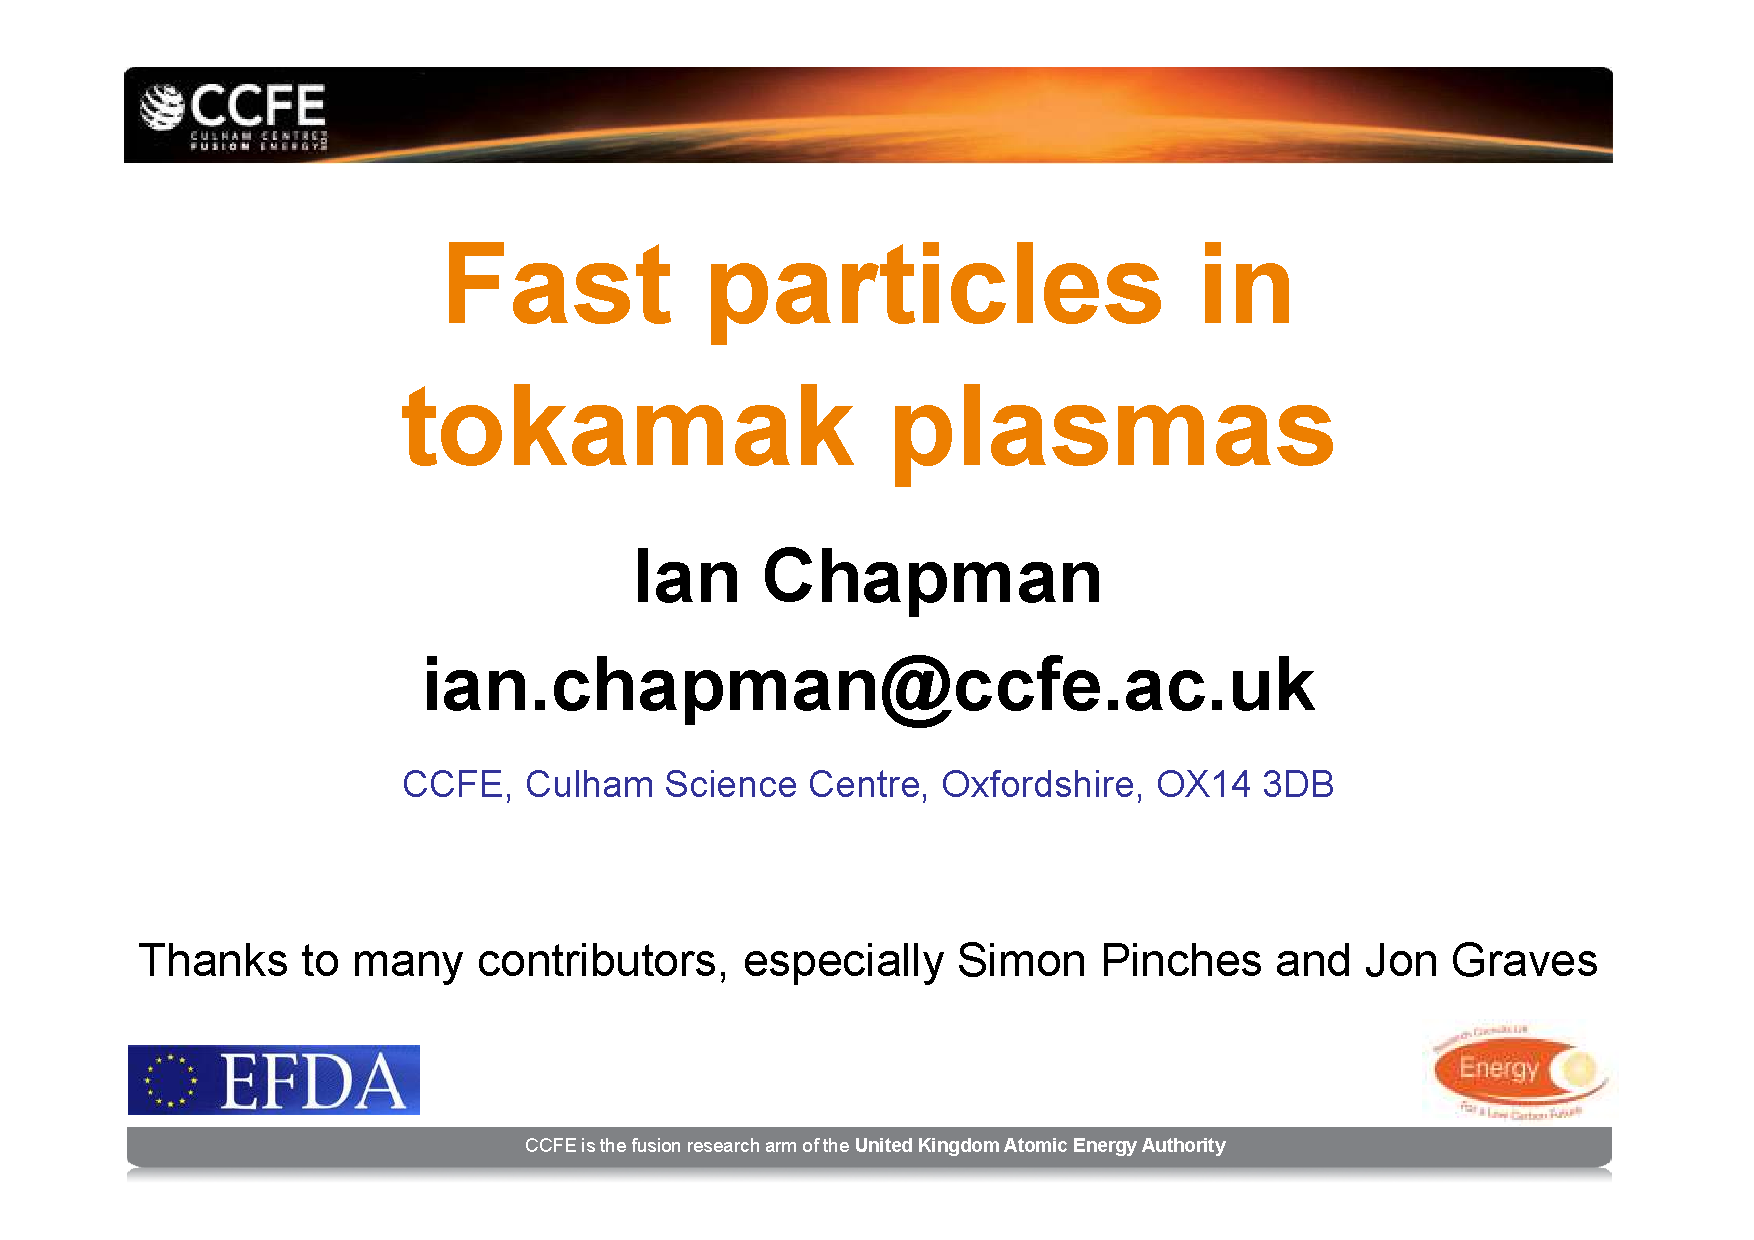
\includegraphics[scale=0.5]{trapped_particles.png}
\par\end{centering}
\caption{(a) Trapped and (b) passing particles in the view of the poloidal cross-section of tokamaks.}
\label{fig:trapped_particles}
\end{figure}
%%%%%%%%%%%%%%%%%%%%


\subsection{Heating scenarios}

As discussed in section \ref{sec:principles_fusion}, in self-burning fusion plasmas, the radiation power losses are balanced by the heating from the slowing down of the $\alpha$ particles. However, external heating is required in two situations:%
%%%%%%%%%%%%%%%%%%%%
\begin{itemize}

  \item At the initial stage to ignite the reaction.

  \item In experimental plasma studies when the number of fusion reactions is negligible or the power output from the $\alpha$ particles is not enough to compensate the losses.

\end{itemize}
%%%%%%%%%%%%%%%%%%%%
\noindent In tokamaks, the fundamental heating method is Ohmic heating by the large toroidal plasma current through the Joule effect. The Ohmic heating power density is $p_{\mathrm{Ohmic}} = \eta j^2$, where $\eta$ and $j$ are the plasma resistivity and the current density, respectively. Although the intrinsic Ohmic heating is strong at low temperatures, it becomes less efficient at high temperatures, since $\eta$ decreases rapidly with temperature ($\eta \propto T_e^{-3/2}$). Therefore, auxiliary heating methods are required.


There have been mainly two auxiliary heating methods: the injection of energetic neutral beams and the resonant energy absorption of electromagnetic fields in the radio-frequency (RF) domain. Both methods can provide power levels of the order of MW. Neutral beam injection (NBI) heats both electrons and ions through Coulomb collisions between the neutral particles and the charged plasma particles. The RF heating can be further categorized into three types according to their frequencies:%
%%%%%%%%%%%%%%%%%%%%
\begin{itemize}

  \item Ion cyclotron resonance heating (ICRH) transfers the energy of the electromagnetic waves to ions at the resonance condition $\omega = \omega_{ci}$ (in tens of MHz).

  \item Electron cyclotron resonance heating (ECRH) directly heats the electrons through microwaves in the frequency range of hundred of GHz.

  \item Lower-hybrid (LH) heating uses electromagnetic waves in the frequency range 1-8 GHz, which is between the ion and electron cyclotron frequency: $\omega_{ci} < \omega < \omega_{ce}$. LH heating is particularly useful for current drive because of its effect on current profiles. LH heating is also the conventional heating method in long-pulse operations.

\end{itemize}
%%%%%%%%%%%%%%%%%%%%

The development of heating scenarios contributes to accomplishing the goals of tokamak experiments in several ways. Most importantly, auxiliary heating allows reaching the power threshold to trigger the transition from the low-confinement regime (L-mode) to high-confinement regime (H-mode). However, in auxiliary heated plasmas, the dynamics of the charged particles becomes even more complicated because, energetic particles form after gaining kinetic energy from the injected electromagnetic waves or beams. The energetic particles can further drive various instabilities. Specifically, ECRH and LH heating could generate fast electrons, which can further drive the electron fishbone instabilities. ICRH and NBI give rise to different types of instabilities such as the energetic-ion-driven Alfv\'{e}n waves.


\subsection{Basic diagnostics}

In tokamaks, various diagnostics have been developed to measure the basic plasma parameters \cite{Hutchinson_2002_Diagnostics,Wesson_1997_Tokamaks}. First of all, magnetic loops or coils provide the most fundamental plasma properties such as the plasma current ($I_p$), loop voltage ($V_p$), plasma position and shape (elongation, triangularity), plasma energy (W), etc. Specifically, the energy confinement time can be obtained by the ratio between the plasma energy and the input heating power: $\tau_E = W/P_\mathrm{input}$.

The basic plasma parameters include the electron density ($n_e$) and the electron temperature ($T_e$). Interferometry has been a standard tool to measure the line integral of the electron density by the phase difference between the measuring beam and the reference beam. Multiple channels (arrays) of interferometry measurements combined with an inversion technique can provide the local $n_e$ profile in a poloidal cross-section, with a spatial resolution depending on the number and coverage of the set of chords. A reflectometry diagnostic measures the reflected part of an emitted wave to provide the local $n_e$ with a much higher spatial resolution, as discussed in more detail in chapter \ref{ch:Reflectometry}. Two different methods have been developed to measure the electron temperature in tokamaks: Thomson scattering and electron cyclotron emission (ECE). Thomson scattering directly measures the plasma pressure ($n_e$, $T_e$) by actively launching laser beams into the plasma and spectrum broadening of the scattered beams provides $T_e$, whereas ECE determines $T_e$ by passively measuring the intensity of harmonic frequencies of electron cyclotron emission ($\omega = n\omega_{ce}$, $n$ the harmonic number, $\omega_{ce}$ the electron cyclotron frequency). Although both methods can provide the radial profile of $T_e$, Thomson scattering can also provide the accurate edge values where the plasma optical depth is not sufficient to obtain an accurate $T_e$ estimation by ECE. On the other hand, ECE has a much higher temporal resolution with lower noise, which can be used to study the fast physical process such as the sawtooth instability. Although Langmuir probes can usually provide accurate measurements of $n_e$ and $T_e$, their application is constrained to the edge region where the temperature does not exceed the capability of the probes.

Information about the ion properties, including the ion temperature ($T_i$) and the effective charge number ($Z_\mathrm{eff}$) is also important. $T_i$ is generally estimated from the Doppler broadening of line radiation from charge exchange recombination spectroscopy (CXRS). $Z_\mathrm{eff}$ is a measure of the degree of impurity, defined as $Z_\mathrm{eff} = \sum n_iZ_i^2/n_e$, where $Z_i$ is the charge number of each ion species. In a fully ionized pure hydrogen isotope plasma, $Z_\mathrm{eff} = 1$, and normally $Z_\mathrm{eff} > 1$. Measurement of bremsstrahlung radiation is typically used to estimate $Z_\mathrm{eff}$.


\subsection{Tore Supra}

Since this thesis is totally based on the database of the Tore Supra tokamak, which was located in the Institute for Magnetic Fusion Research (IRFM) at CEA Cadarache in Southern France, the basic parameters, heating methods and diagnostics of Tore Supra are briefly introduced.


Tore Supra (from "torus" and "superconductor") operated from 1988 to 2011 and has in the meantime been upgraded to the WEST machine (Tungsten Environment in Steady-state Tokamak), since 2016. Tore Supra had a circular cross-section with actively cooled plasma-facing components and a set of pump limiters. Equipped with superconducting toroidal magnets, it was initially developed to investigate technical and physical issues in long-pulse steady-state plasmas. Tore Supra once held the world record for the longest tokamak pulse (6 mins 30 secs) in 2003. Table \ref{tab:ts_parameters} lists some typical values of basic operational parameters of Tore Supra. Tore Supra was a conventional tokamak ($R_p \gg a$) operating at high magnetic fields ($> 3$ T) with relatively long plasma pulses ($> 10$ s).


%%%%%%%%%%%%%%%%%%%%
\begin{table}[h]
\begin{center}
\begin{tabular}{|c|c|}
  \hline \hline
  % after \\: \hline or \cline{col1-col2} \cline{col3-col4} ...
  On-axis toroidal magnetic field $B_{0}$ & 3.4/3.8 T \\ \hline
  Plasma current $I_p$ & 1 MA \\ \hline
  Major radius $R_{p}$ & 2.38 m \\ \hline
  Minor radius $a$ & 0.72 m \\ \hline
  Plasma elongation $\kappa$ & 1.0 \\ \hline
  Line-averaged electron density $\langle{n_e}\rangle$ & $2 \times 10^{-19}\ m^{-3}$ \\ \hline
  Central line-integrated density $n_{l}$ & $4 \times 10^{-19}\ m^{-2}$ \\ \hline
  Plasma volume & 25 m$^3$ \\ \hline
  Pulse duration & 20 s \\
  \hline \hline
\end{tabular}
\caption{Typical operational parameters of the Tore Supra tokamak.}
\label{tab:ts_parameters}
\end{center}
\end{table}
%%%%%%%%%%%%%%%%%%%%


Tore Supra was equipped with lower hybrid current drive (LHCD), ICRH and ECRH systems, the locations of which are shown in figure \ref{fig:ts_heating}. The 3.7 GHz LHCD system was designed to inject 8 MW of additional power in long-pulse operations \cite{Bibet_2001_FED}. Note that LHCD can generate suprathermal electrons, which could increase the parasitic noise of some diagnostic measurements. ICRH is another main auxiliary heating system on Tore Supra and its operational frequencies are between 35 MHz to 80 MHz. Three ICRH antennas were installed in port Q1, Q2 and Q5, respectively (figure \ref{fig:ts_heating}), and the antenna positions were kept almost constant. Each antenna can inject up to 4 MW power \cite{Colas_2006_NF_ICRH}. ECRH heats the electrons by microwaves at the frequency of 118 GHz, generated by 2 gyrotrons of 400 kW \cite{Lennholm_2003_NF_ECRH}. However, due to technical problems, the number of ECRH plasmas is relatively limited in the Tore Supra database.


%%%%%%%%%%%%%%%%%%%%
\begin{figure}[h]
\begin{centering}
\includegraphics[scale=0.7]{ts_heating.png}
\par\end{centering}
\caption{The locations of the LHCD, ICRH and ECRH systems installed at Tore Supra from the top view.}
\label{fig:ts_heating}
\end{figure}
%%%%%%%%%%%%%%%%%%%%

The details of the Tore Supra diagnostics can be found in \cite{Gil_2009_FST}. For the basic parameters, a 10-channel far-infrared interferometry system was installed to measure the radial profile of $n_e$ with 1 ms time resolution. However, measurements of edge density have larger uncertainties due to the lack of spatial points in the strong $\nabla n$ region. A 32-channel ECE system \cite{Segui_2005_RSI} was installed to measure the radial profile of $T_e$ with both slow (1 ms) and fast (1 $\mu$s) acquisition and spatial resolution of 2 $-$ 3 cm. $T_i$ was measured from CXRS but only in a very limited number of discharges. $Z_\mathrm{eff}$ was measured by bremsstrahlung in both vertical and tangential directions. More dedicated diagnostics have been designed for various specific physics studies such as turbulence research. Three reflectometry systems, viz. the D-band core fixed-frequency reflectometer \cite{Sabot_2006_NF}, the V- and W-band edge fast-sweeping reflectometer \cite{Clairet_2010_RSI} and the Doppler reflectometer \cite{Hennequin_2006_NF} (discussed in more detail in chapter \ref{ch:Reflectometry}) enable a comprehensive study of density turbulence from the edge to the core region.


\section{Motivation of this thesis} \label{sec:motivation_thesis}


The motivation of this thesis is related to both the issue of plasma turbulence and the methodology for extracting information about the turbulence. The unsolved problems of turbulent fluctuations and their link with micro-instabilities and transport have essentially driven the turbulence study for this thesis (as well as many other theses). The specificity of this thesis lies in the fact that it is the first attempt of a database approach in the context of fusion turbulence studies. A systematic study is possible thanks to the large amount of accumulated experimental data over many years of operation of Tore Supra. In addition, a dedicated methodology was developed to enable such a study, using methods from the field of probability and statistics.



\subsection{Gradient-driven turbulence}

In tokamak fusion plasmas, the electron density $n_e$ and temperature $T_e$ are very high in the core region. The typical $n_e$ and $T_e$ are $1\times 10^{20}\ m^{-3}$ and $10\ keV$, respectively. However, in the edge plasma near the wall, $n_e$ and $T_e$ decrease to the order of $10^{17}\ m^{-3}$ and $10\ eV$, respectively, to avoid excessive heat and particle loads on the wall. Figure \ref{fig:gradient} illustrates the large disparity of $n_e$ and $T_e$ in the central and edge regions, as well as the typical electron density profile $n_e(r)$ and temperature profile $T_e(r)$. A region with strong gradient of $n_e$, $T_e$, and thus pressure gradient ($p = nKT$, $K$ the Boltzmann constant), exists between the central and edge regions. This strong gradient provides the free energy to create micro-instabilities which can develop into the saturation state called \emph{turbulence}. Furthermore, particles and energy can transfer across the turbulent vortices rapidly. Consequently, the cross-field transport increases and the confinement degrades.


%%%%%%%%%%%%%%%%%%%%
\begin{figure}[h]
\begin{centering}
\includegraphics[scale=1]{gradient.png}
\par\end{centering}
\caption[Gradient from core to edge]{Strong $n_e$ and $T_e$ gradient between the central and edge region of tokamaks.}
\label{fig:gradient}
\end{figure}
%%%%%%%%%%%%%%%%%%%%


Experimentally, many diagnostics and analysis methods have been developed to measure the fluctuations of density ($\tilde{n}$), temperature ($\tilde{T}$), electric potential ($\tilde{\phi}$) and magnetic field ($\tilde{\bu{B}}$) originating from plasma turbulence. The relations between turbulence and transport are also unclear so far. Since turbulence has deleterious effects on the confinement, it is very important to understand the underlying physics of the instabilities, turbulence, and turbulent transport.


%%%%%%%%%%%%%%%%%%%%%
%\begin{figure}[h]
%\begin{centering}
%\includegraphics[scale=0.8]{process.png}
%\par\end{centering}
%\caption{Simplified physics process of the turbulence and transport processes.}
%\label{fig:process}
%\end{figure}
%%%%%%%%%%%%%%%%%%%%%


\subsection{Towards a systematic study}


The fixed-frequency reflectometry on Tore Supra has been dedicated to detect local turbulence properties in the core region. After years of measurements, a large reflectometry database covering a wide range of plasma conditions has been obtained. This drives this thesis to carry out a database study of plasma turbulence by systematic analysis of the frequency spectra obtained from the reflectometry measurements in order to find more general trends or patterns.


This systematic study originates from the extensive application of data science, involving methods from probability theory, statistics, machine learning, etc., throughout science and engineering. In fusion research,the global energy confinement time \cite{Greenwald_1984_PRL} or the power threshold for the transition from low to high confinement \cite{Martin_2008_JoP} are two well-known examples of database analysis. Trends are often described in terms of other quantities through semi-empirical scaling laws \cite{Yushmanov_1990_NF,Verdoolaege_2015_NF}. The parameters of these scaling laws, estimated using statistical regression methods, are instructive to the underlying turbulent transport properties and micro-instabilities. A database approach with statistical tools can be very useful for making an inventory of the characteristics of some aspects of the plasma, allowing investigations of systematic trends that could remain hidden in smaller-scale studies. Although physical explanation of observed trends is not always straightforward, knowledge of trends can drive the development of physical models, contribute to their verification and enable predictions.


A database approach is complementary to the more traditional shot-to-shot analysis, the latter involving a more strictly controlled range of plasma conditions and accurate measurements. The shot-to-shot analysis is usually supported by simulations to interpret the experimental observations, which in turn help to validate the simulation models and tools for dedicated discharges \cite{White_2008_PoP,Sung_2016_PoP,Holland_2016_PoP,Creely_2017_PoP}. However, undertaking systematic simulations for even a part of a database may be hampered by prohibitive computing time and human resources. On the other hand, trends identified through a database analysis can lead to new experimental proposals and shot-to-shot analysis to explain or confirm the trends. For instance, in the dimensionless energy confinement time scaling law \cite{Petty_1995_PoP}, the dependence of confinement on the normalized Larmor radius can give clues on the Bohm or gyro-Bohm scaling of the turbulent eddies. This dependence has also been investigated through dedicated Larmor scaling experiments \cite{Christiansen_1993_NF,Vlad_2005_PPCF}.


Furthermore, in the majority of studies of trends in fusion science, the response variable is usually a single scalar quantity, such as the energy confinement time or power threshold for the transition from low to high confinement. However, this study aims at characterizing frequency spectra by multiple quantities, such as the spectrum shape, width, components, etc. In order to make the problem manageable, each spectrum has to be described using a sufficiently succinct model, that captures the essential characteristics of the spectrum. Since the frequency spectrum obtained by the Fourier transform algorithm requires several hundreds to a thousand frequency bins for a good spectral resolution, some kind of dimensionality reduction is needed, in order to decrease the number of parameters used to describe each spectrum. The earlier work regarding frequency spectrum decomposition \cite{Vershkov_2005_NF,Vershkov_2011_NF, Kramer-Flecken_2004_NF,Kramer-Flecken_2015_NJP}, as shown in figure \ref{fig:decomposition}, inspires us to further parameterize the spectra by a few parameters. With the few identified turbulence parameters, we will be able to investigate globally the turbulence properties in different plasmas heating scenarios and extract the general trends. The realization process of this database turbulence analysis is shown in figure \ref{fig:objective}, which contains the main work of this thesis.


%%%%%%%%%%%%%%%%%%%%
\begin{figure}[h]
\begin{centering}
\includegraphics[scale=0.52]{decomposition.png}
\par\end{centering}
\caption{Spectrum decomposition by (a) the power spectrum from \cite{Vershkov_2005_NF} and (b) the coherence spectrum from \cite{Kramer-Flecken_2015_NJP}.}
\label{fig:decomposition}
\end{figure}
%%%%%%%%%%%%%%%%%%%%



%%%%%%%%%%%%%%%%%%%%
\begin{figure}[h]
\begin{centering}
\includegraphics[scale=0.65]{objective.png}
\par\end{centering}
\caption{The process of a systematic turbulence study from frequency spectra of density fluctuation measurements by fixed-frequency reflectometry.}
\label{fig:objective}
\end{figure}
%%%%%%%%%%%%%%%%%%%%



\subsection{Outline of this thesis}

As this study has been focused on a systematic study of frequency spectra from reflectometry fluctuation measurements, chapters 2 and 3 are dedicated to a detailed discussion on turbulence and reflectometry before carrying on with the actual thesis work:%
%%%%%%%%%%%%%%%%%%%%
\begin{itemize}

  \item \textbf{Chapter 2} starts from the general properties of turbulent phenomena before focusing on the turbulent transport in magnetic confinement devices. We then introduce the origin of turbulence in tokamak fusion plasmas from micro-instabilities, focusing on TEM and ITG instabilities and the effects of collisionality. Finally, some properties of the density fluctuations are presented.

  \item \textbf{Chapter 3} first derives the dispersion relation from the classical theory of electromagnetic wave propagation. Next, we focus on the effects of turbulent fluctuations on electromagnetic wave propagation. Then, the principles of reflectometry for both profile and fluctuation measurements are presented, based on the concept of wave reflection on plasma cut-off layers. The fixed-frequency reflectometer used in this thesis is then introduced.

\end{itemize}
%%%%%%%%%%%%%%%%%%%%
\noindent After the introduction of turbulence and reflectometry, the main studies of this thesis are included in chapters 4--6:%
%%%%%%%%%%%%%%%%%%%%
\begin{itemize}

  \item \textbf{Chapter 4} is dedicated to the parametrization of the fluctuation frequency spectra, focusing on the optimization of the spectrum fitting process. Different fitting models will be compared..

  \item \textbf{Chapter 5} focuses on the radial profiles of the broadband fraction of the frequency spectra in both Ohmic and L-mode plasmas. In the end, a link between the broadband fraction and the density fluctuation level is developed.

  \item \textbf{Chapter 6} discusses collisional effects on the frequency spectra in Ohmic and L-mode plasmas. We then propose an interpretation in terms of a transition of the dominating instability, supported by earlier gyrokinetic simulations, to explain the observed results. Further evidence is provided by analysis of the density peaking and study of the low-frequency components of the spectra.

\end{itemize}
%%%%%%%%%%%%%%%%%%%%
\noindent Finally, \textbf{chapter 7} summarizes the main results and provides conclusions of this thesis. Some pending issues and motivation for future work is discussed.
